\frame
{
	\frametitle{Our Method}
	\begin{enumerate}
	\item Initialize a set of paths $\mathcal{P}$~(in polynomial size).
	\vspace{0.2cm}
	\item Use LP to estimate the abundance of the paths in $\mathcal{B}$ to minimize the estimation error.
	\vspace{0.2cm}
	\item Reduce the number of paths in $\mathcal{P}$:
		\begin{itemize}
		\vspace{0.1cm}
		\item For two paths with (almost) identical abundance, try to merge them into one path;
		\vspace{0.1cm}
		\item Discard paths with very small abundance.
		\end{itemize}
	\vspace{0.2cm}
	\item Iterate between step 2 and step 3.
	\end{enumerate}
}

\frame
{
	\frametitle{Bad Example for Greedy Algorithm}

	\vspace{0.2cm}
	\begin{center}

\begin{tikzpicture}[font=\small,overlay,
mycirclex/.style={draw, circle, minimum size=1.0em, inner sep = 0.2mm}, 
mydiamond/.style={draw, diamond, minimum size=0.78em, inner sep = 0mm}, 
myrectang/.style={draw, rectangle, minimum size=0.60em, inner sep = 0mm}, 
>=stealth]

\definecolor{mygreen}{rgb}{0, 0.7, 0}
\definecolor{myyellow}{rgb}{0.8, 0.6, 0}

\def\colx{black}
\def\cola{red} 
\def\colb{blue}
\def\colc{violet}
\def\cold{cyan} 
\def\cole{myyellow}
\def\colf{brown}


\def\len{1.8cm}

% G1
\begin{scope}[local bounding box=bbox, xshift=-6.4cm, yscale=1.2]
\path<2-> node[mycirclex] (v1) at (1.0 * \len, 0) {$s$};
\path<2-> node[mycirclex] (v2) at (2.0 * \len, 0) {$a$};
\path<2-> node[mycirclex] (v3) at (3.0 * \len, 0) {$b$};
\path<2-> node[mycirclex] (v4) at (4.0 * \len, 0) {$c$};
\path<2-> node[mycirclex] (v5) at (5.0 * \len, 0) {$d$};
\path<2-> node[mycirclex] (v6) at (6.0 * \len, 0) {$t$};

\path<3-> [draw, opacity = 1.0, \cola, ->, line width=0.082cm] (v1) -- (v2);
\path<3-> [draw, opacity = 1.0, \cola, ->, line width=0.082cm] (v2) -- (v3);
\path<3-> [draw, opacity = 1.0, \cola, ->, line width=0.082cm] (v3) -- (v4);
\path<3-> [draw, opacity = 1.0, \cola, ->, line width=0.082cm] (v4) -- (v5);
\path<3-> [draw, opacity = 1.0, \cola, ->, line width=0.082cm] (v5) -- (v6);
\path<4-> [draw, \colb, opacity = 1.0, ->, line width=0.082cm, bend left = 50] (v1) to (v2);
\path<4-> [draw, \colb, opacity = 1.0, ->, line width=0.082cm, bend left = 30] (v3) to (v6);
\path<4-> [draw, \colb, opacity = 1.0, ->, line width=0.082cm, bend left =-20] (v2) to (v3);
\path<5-> [draw, \colc, opacity = 1.0, ->, line width=0.082cm, bend left = 50] (v5) to (v6);
\path<5-> [draw, \colc, opacity = 1.0, ->, line width=0.082cm, bend left = 30] (v1) to (v4);
\path<5-> [draw, \colc, opacity = 1.0, ->, line width=0.082cm, bend left =-20] (v4) to (v5);

\path<2-> [draw, \colx, ->, line width=0.02cm] (v1) -- (v2);
\path<2-> [draw, \colx, ->, line width=0.02cm] (v2) -- (v3);
\path<2-> [draw, \colx, ->, line width=0.02cm] (v3) -- (v4);
\path<2-> [draw, \colx, ->, line width=0.02cm] (v4) -- (v5);
\path<2-> [draw, \colx, ->, line width=0.02cm] (v5) -- (v6);

\path<2-> [draw, \colx, ->, line width=0.02cm, bend left = 50] (v1) to (v2);
\path<2-> [draw, \colx, ->, line width=0.02cm, bend left = 50] (v5) to (v6);
\path<2-> [draw, \colx, ->, line width=0.02cm, bend left = 30] (v1) to (v4);
\path<2-> [draw, \colx, ->, line width=0.02cm, bend left = 30] (v3) to (v6);

\path<2-> [draw, \colx, ->, line width=0.02cm, bend left =-20] (v2) to (v3);
\path<2-> [draw, \colx, ->, line width=0.02cm, bend left =-30] (v2) to (v3);
\path<2-> [draw, \colx, ->, line width=0.02cm, bend left =-40] (v2) to (v3);
\path<2-> [draw, \colx, ->, line width=0.02cm, bend left =-50] (v2) to (v3);
\path<2-> [draw, \colx, ->, line width=0.02cm, bend left =-20] (v4) to (v5);
\path<2-> [draw, \colx, ->, line width=0.02cm, bend left =-30] (v4) to (v5);
\path<2-> [draw, \colx, ->, line width=0.02cm, bend left =-40] (v4) to (v5);
\path<2-> [draw, \colx, ->, line width=0.02cm, bend left =-50] (v4) to (v5);


\path<2-> node at (1.5 * \len, 0.17cm) {$2n$};
\path<2-> node at (2.5 * \len, 0.17cm) {$2n$};
\path<2-> node at (3.5 * \len, 0.17cm) {$2n$};
\path<2-> node at (4.5 * \len, 0.17cm) {$2n$};
\path<2-> node at (5.5 * \len, 0.17cm) {$2n$};

\path<2-> node at (1.4 * \len, 0.62cm) {$n$};
\path<2-> node at (5.6 * \len, 0.62cm) {$n$};
\path<2-> node at (2.5 * \len, 0.96cm) {$n$};
\path<2-> node at (4.5 * \len, 0.96cm) {$n$};

\path<2-> node at (2.5 * \len, -0.65cm) {$n\times 1$};
\path<2-> node at (4.5 * \len, -0.65cm) {$n\times 1$};
\end{scope}


\end{tikzpicture}
\end{center}

	\vspace{0.8cm}
	\onslide<6->{{\bf Solution by greedy algorithm:} $2n + 1$ paths.}

	\vspace{1.5cm}
	\begin{center}


\begin{tikzpicture}[font=\small,overlay,
mycirclex/.style={draw, circle, minimum size=1.0em, inner sep = 0.2mm}, 
mydiamond/.style={draw, diamond, minimum size=0.78em, inner sep = 0mm}, 
myrectang/.style={rounded corners, draw, rectangle, minimum size=0.60em, inner sep = 0.8mm, line width = 0.03cm}, 
>=stealth]

\definecolor{mygreen}{rgb}{0, 0.7, 0}
\definecolor{myyellow}{rgb}{0.8, 0.6, 0}

\def\colx{black}
\def\cola{red} 
\def\colb{blue}
\def\colc{violet}
\def\cold{cyan} 
\def\cole{myyellow}
\def\colf{brown}


\def\len{1.65cm}

% G1
\begin{scope}[local bounding box=bbox, xshift=-6.9cm, yscale=1.2]
\path<7-> node[mycirclex] (v1) at (1.0 * \len, 0) {$s$};
\path<7-> node[mycirclex] (v2) at (2.0 * \len, 0) {$a$};
\path<7-> node[mycirclex] (v3) at (3.0 * \len, 0) {$b$};
\path<7-> node[mycirclex] (v4) at (4.0 * \len, 0) {$c$};
\path<7-> node[mycirclex] (v5) at (5.0 * \len, 0) {$d$};
\path<7-> node[mycirclex] (v6) at (6.0 * \len, 0) {$t$};

\path<11-> [draw, \cold, ->, line width=0.122cm, bend left = 50] (v1) to (v2);
\path<11-> [draw, \cold, ->, line width=0.122cm, bend left =-20] (v2) to (v3);
\path<11-> [draw, \cold, ->, line width=0.122cm, bend left =-20] (v4) to (v5);
\path<11-> [draw, \cold, ->, line width=0.122cm, bend left = 50] (v5) to (v6);
\path<11-> [draw, \cold, ->, line width=0.122cm] (v3) -- (v4);
\path<11-> node[myrectang, rounded corners, \cold] at (7 * \len, -0.75cm) {$a(P_4) = 1~(\times n)$};

\path<10-> [draw, \colc, ->, line width=0.122cm, bend left = 30] (v1) to (v4);
\path<10-> [draw, \colc, ->, line width=0.122cm] (v4) -- (v5);
\path<10-> [draw, \colc, ->, line width=0.122cm] (v5) -- (v6);
\path<10-> node[myrectang, rounded corners, \colc] at (7 * \len, -0.25cm) {$a(P_3) = n~(\times 1)$};

\path<9-> [draw, \colb, ->, line width=0.122cm] (v1) -- (v2);
\path<9-> [draw, \colb, ->, line width=0.122cm] (v2) -- (v3);
\path<9-> [draw, \colb, ->, line width=0.122cm, bend left = 30] (v3) to (v6);
\path<9-> node[myrectang, rounded corners, \colb] at (7 * \len, 0.25cm) {$a(P_2) = n~(\times 1)$};


\path<8-> [draw, \cola, ->, line width=0.052cm] (v1) -- (v2);
\path<8-> [draw, \cola, ->, line width=0.052cm] (v2) -- (v3);
\path<8-> [draw, \cola, ->, line width=0.052cm] (v3) -- (v4);
\path<8-> [draw, \cola, ->, line width=0.052cm] (v4) -- (v5);
\path<8-> [draw, \cola, ->, line width=0.052cm] (v5) -- (v6);
\path<8-> node[myrectang, rounded corners, \cola] at (7 * \len, 0.75cm) {$a(P_1) = n~(\times 1)$};

\path<7-> [draw, \colx, ->, line width=0.02cm] (v1) -- (v2);
\path<7-> [draw, \colx, ->, line width=0.02cm] (v2) -- (v3);
\path<7-> [draw, \colx, ->, line width=0.02cm] (v3) -- (v4);
\path<7-> [draw, \colx, ->, line width=0.02cm] (v4) -- (v5);
\path<7-> [draw, \colx, ->, line width=0.02cm] (v5) -- (v6);

\path<7-> [draw, \colx, ->, line width=0.02cm, bend left = 50] (v1) to (v2);
\path<7-> [draw, \colx, ->, line width=0.02cm, bend left = 50] (v5) to (v6);
\path<7-> [draw, \colx, ->, line width=0.02cm, bend left = 30] (v1) to (v4);
\path<7-> [draw, \colx, ->, line width=0.02cm, bend left = 30] (v3) to (v6);

\path<7-> [draw, \colx, ->, line width=0.02cm, bend left =-20] (v2) to (v3);
\path<7-> [draw, \colx, ->, line width=0.02cm, bend left =-30] (v2) to (v3);
\path<7-> [draw, \colx, ->, line width=0.02cm, bend left =-40] (v2) to (v3);
\path<7-> [draw, \colx, ->, line width=0.02cm, bend left =-50] (v2) to (v3);
\path<7-> [draw, \colx, ->, line width=0.02cm, bend left =-20] (v4) to (v5);
\path<7-> [draw, \colx, ->, line width=0.02cm, bend left =-30] (v4) to (v5);
\path<7-> [draw, \colx, ->, line width=0.02cm, bend left =-40] (v4) to (v5);
\path<7-> [draw, \colx, ->, line width=0.02cm, bend left =-50] (v4) to (v5);


\path<7-> node at (1.5 * \len, 0.17cm) {$2n$};
\path<7-> node at (2.5 * \len, 0.17cm) {$2n$};
\path<7-> node at (3.5 * \len, 0.17cm) {$2n$};
\path<7-> node at (4.5 * \len, 0.17cm) {$2n$};
\path<7-> node at (5.5 * \len, 0.17cm) {$2n$};

\path<7-> node at (1.4 * \len, 0.62cm) {$n$};
\path<7-> node at (5.6 * \len, 0.62cm) {$n$};
\path<7-> node at (2.5 * \len, 0.96cm) {$n$};
\path<7-> node at (4.5 * \len, 0.96cm) {$n$};

\path<7-> node at (2.5 * \len, -0.65cm) {$n\times 1$};
\path<7-> node at (4.5 * \len, -0.65cm) {$n\times 1$};
\end{scope}


\end{tikzpicture}
\end{center}

	\vspace{0.8cm}
	\onslide<12->{{\bf Optimal solution:} $n + 3$ paths.}
}

\frame
{
	\frametitle{Use the Residual Graph}

	\vspace{-3.4cm}
	\begin{center}

\begin{tikzpicture}[font=\small,overlay,
mycirclex/.style={draw, circle, minimum size=1.0em, inner sep = 0.2mm}, 
mydiamond/.style={draw, diamond, minimum size=0.78em, inner sep = 0mm}, 
myrectang/.style={rounded corners, draw, rectangle, minimum size=0.60em, inner sep = 0.8mm, line width = 0.03cm}, 
>=stealth]

\definecolor{mygreen}{rgb}{0, 0.7, 0}
\definecolor{myyellow}{rgb}{0.8, 0.6, 0}

\def\colx{black}
\def\cola{red} 
\def\colb{blue}
\def\colc{violet}
\def\cold{cyan} 
\def\cole{myyellow}
\def\colf{brown}


\def\len{1.65cm}

% G1
\begin{scope}[local bounding box=bbox, xshift=-6.9cm, yscale=1.2]
\path<2-> node[mycirclex] (v1) at (1.0 * \len, 0) {$s$};
\path<2-> node[mycirclex] (v2) at (2.0 * \len, 0) {$a$};
\path<2-> node[mycirclex] (v3) at (3.0 * \len, 0) {$b$};
\path<2-> node[mycirclex] (v4) at (4.0 * \len, 0) {$c$};
\path<2-> node[mycirclex] (v5) at (5.0 * \len, 0) {$d$};
\path<2-> node[mycirclex] (v6) at (6.0 * \len, 0) {$t$};

\path<3-> [draw, opacity = 1.0, \cola, ->, line width=0.082cm] (v1) -- (v2);
\path<3-> [draw, opacity = 1.0, \cola, ->, line width=0.082cm] (v2) -- (v3);
\path<3-> [draw, opacity = 1.0, \cola, ->, line width=0.082cm] (v3) -- (v4);
\path<3-> [draw, opacity = 1.0, \cola, ->, line width=0.082cm] (v4) -- (v5);
\path<3-> [draw, opacity = 1.0, \cola, ->, line width=0.082cm] (v5) -- (v6);
\path<3-> node[myrectang, rounded corners, \cola] at (7.03 * \len, 0.0cm) {$a(P_1) = 2n~(\times 1)$};

\path<2-> [draw, \colx, ->, line width=0.02cm] (v1) -- (v2);
\path<2-> [draw, \colx, ->, line width=0.02cm] (v2) -- (v3);
\path<2-> [draw, \colx, ->, line width=0.02cm] (v3) -- (v4);
\path<2-> [draw, \colx, ->, line width=0.02cm] (v4) -- (v5);
\path<2-> [draw, \colx, ->, line width=0.02cm] (v5) -- (v6);

\path<2-> [draw, \colx, ->, line width=0.02cm, bend left = 50] (v1) to (v2);
\path<2-> [draw, \colx, ->, line width=0.02cm, bend left = 50] (v5) to (v6);
\path<2-> [draw, \colx, ->, line width=0.02cm, bend left = 30] (v1) to (v4);
\path<2-> [draw, \colx, ->, line width=0.02cm, bend left = 30] (v3) to (v6);

\path<2-> [draw, \colx, ->, line width=0.02cm, bend left =-20] (v2) to (v3);
\path<2-> [draw, \colx, ->, line width=0.02cm, bend left =-30] (v2) to (v3);
\path<2-> [draw, \colx, ->, line width=0.02cm, bend left =-40] (v2) to (v3);
\path<2-> [draw, \colx, ->, line width=0.02cm, bend left =-50] (v2) to (v3);
\path<2-> [draw, \colx, ->, line width=0.02cm, bend left =-20] (v4) to (v5);
\path<2-> [draw, \colx, ->, line width=0.02cm, bend left =-30] (v4) to (v5);
\path<2-> [draw, \colx, ->, line width=0.02cm, bend left =-40] (v4) to (v5);
\path<2-> [draw, \colx, ->, line width=0.02cm, bend left =-50] (v4) to (v5);


\path<2-> node at (1.5 * \len, 0.17cm) {$2n$};
\path<2-> node at (2.5 * \len, 0.17cm) {$2n$};
\path<2-> node at (3.5 * \len, 0.17cm) {$2n$};
\path<2-> node at (4.5 * \len, 0.17cm) {$2n$};
\path<2-> node at (5.5 * \len, 0.17cm) {$2n$};

\path<2-> node at (1.4 * \len, 0.62cm) {$n$};
\path<2-> node at (5.6 * \len, 0.62cm) {$n$};
\path<2-> node at (2.5 * \len, 0.96cm) {$n$};
\path<2-> node at (4.5 * \len, 0.96cm) {$n$};

\path<2-> node at (2.5 * \len, -0.65cm) {$n\times 1$};
\path<2-> node at (4.5 * \len, -0.65cm) {$n\times 1$};

\path<4-> [draw, line width = 0.1cm, ->] (3.5 * \len, -0.7cm) to node[label=right:{Residual Graph}]{} (3.5 * \len, -1.4cm);
\end{scope}

% G2
\begin{scope}[local bounding box=bbox, xshift=-6.9cm, yscale=1.2, yshift=-2.4cm]
\path<4-> node[mycirclex] (v1) at (1.0 * \len, 0) {$s$};
\path<4-> node[mycirclex] (v2) at (2.0 * \len, 0) {$a$};
\path<4-> node[mycirclex] (v3) at (3.0 * \len, 0) {$b$};
\path<4-> node[mycirclex] (v4) at (4.0 * \len, 0) {$c$};
\path<4-> node[mycirclex] (v5) at (5.0 * \len, 0) {$d$};
\path<4-> node[mycirclex] (v6) at (6.0 * \len, 0) {$t$};

\path<5-> [draw, \colb, opacity = 1.0, ->, line width=0.082cm, bend left = 30] (v1) to (v4);
\path<5-> [draw, \colb, opacity = 1.0, <-, line width=0.082cm] (v3) -- (v4);
\path<5-> [draw, \colb, opacity = 1.0, ->, line width=0.082cm, bend left = 30] (v3) to (v6);
\path<5-> node[myrectang, rounded corners, \colb] at (7.03 * \len, 0.0cm) {$a(P_2) = n~(\times 1)$};

\path<4-> [draw, \colx, <-, line width=0.02cm] (v1) -- (v2);
\path<4-> [draw, \colx, <-, line width=0.02cm] (v2) -- (v3);
\path<4-> [draw, \colx, <-, line width=0.02cm] (v3) -- (v4);
\path<4-> [draw, \colx, <-, line width=0.02cm] (v4) -- (v5);
\path<4-> [draw, \colx, <-, line width=0.02cm] (v5) -- (v6);

\path<4-> [draw, \colx, ->, line width=0.02cm, bend left = 50] (v1) to (v2);
\path<4-> [draw, \colx, ->, line width=0.02cm, bend left = 50] (v5) to (v6);
\path<4-> [draw, \colx, ->, line width=0.02cm, bend left = 30] (v1) to (v4);
\path<4-> [draw, \colx, ->, line width=0.02cm, bend left = 30] (v3) to (v6);

\path<4-> [draw, \colx, ->, line width=0.02cm, bend left =-20] (v2) to (v3);
\path<4-> [draw, \colx, ->, line width=0.02cm, bend left =-30] (v2) to (v3);
\path<4-> [draw, \colx, ->, line width=0.02cm, bend left =-40] (v2) to (v3);
\path<4-> [draw, \colx, ->, line width=0.02cm, bend left =-50] (v2) to (v3);
\path<4-> [draw, \colx, ->, line width=0.02cm, bend left =-20] (v4) to (v5);
\path<4-> [draw, \colx, ->, line width=0.02cm, bend left =-30] (v4) to (v5);
\path<4-> [draw, \colx, ->, line width=0.02cm, bend left =-40] (v4) to (v5);
\path<4-> [draw, \colx, ->, line width=0.02cm, bend left =-50] (v4) to (v5);


\path<4-> node at (1.5 * \len, 0.17cm) {$2n$};
\path<4-> node at (2.5 * \len, 0.17cm) {$2n$};
\path<4-> node at (3.5 * \len, 0.17cm) {$2n$};
\path<4-> node at (4.5 * \len, 0.17cm) {$2n$};
\path<4-> node at (5.5 * \len, 0.17cm) {$2n$};

\path<4-> node at (1.4 * \len, 0.62cm) {$n$};
\path<4-> node at (5.6 * \len, 0.62cm) {$n$};
\path<4-> node at (2.5 * \len, 0.96cm) {$n$};
\path<4-> node at (4.5 * \len, 0.96cm) {$n$};

\path<4-> node at (2.5 * \len, -0.65cm) {$n\times 1$};
\path<4-> node at (4.5 * \len, -0.65cm) {$n\times 1$};
\path<6-> [draw, line width = 0.1cm, ->] (3.5 * \len, -0.7cm) to node[label=right:{Residual Graph}]{} (3.5 * \len, -1.4cm);
\end{scope}

% G3
\begin{scope}[local bounding box=bbox, xshift=-6.9cm, yscale=1.2, yshift=-4.8cm]
\path<6-> node[mycirclex] (v1) at (1.0 * \len, 0) {$s$};
\path<6-> node[mycirclex] (v2) at (2.0 * \len, 0) {$a$};
\path<6-> node[mycirclex] (v3) at (3.0 * \len, 0) {$b$};
\path<6-> node[mycirclex] (v4) at (4.0 * \len, 0) {$c$};
\path<6-> node[mycirclex] (v5) at (5.0 * \len, 0) {$d$};
\path<6-> node[mycirclex] (v6) at (6.0 * \len, 0) {$t$};

\path<7-> [draw, \cold, ->, line width=0.082cm, bend left = 50] (v1) to (v2);
\path<7-> [draw, \cold, ->, line width=0.082cm, bend left =-20] (v2) to (v3);
\path<7-> [draw, \cold, ->, line width=0.082cm, bend left = 10] (v3) to (v4);
\path<7-> [draw, \cold, ->, line width=0.082cm, bend left =-20] (v4) to (v5);
\path<7-> [draw, \cold, ->, line width=0.082cm, bend left = 50] (v5) to (v6);
\path<7-> node[myrectang, rounded corners, \cold] at (7.03 * \len, 0.0cm) {$a(P_3) = 1~(\times n)$};

\path<6-> [draw, \colx, <-, line width=0.02cm] (v1) -- (v2);
\path<6-> [draw, \colx, <-, line width=0.02cm] (v2) -- (v3);
\path<6-> [draw, \colx, <-, line width=0.02cm] (v4) -- (v5);
\path<6-> [draw, \colx, <-, line width=0.02cm] (v5) -- (v6);

\path<6-> [draw, \colx, ->, line width=0.02cm, bend left = 10] (v3) to (v4);
\path<6-> [draw, \colx, <-, line width=0.02cm, bend left =-10] (v3) to (v4);

\path<6-> [draw, \colx, ->, line width=0.02cm, bend left = 50] (v1) to (v2);
\path<6-> [draw, \colx, ->, line width=0.02cm, bend left = 50] (v5) to (v6);
\path<6-> [draw, \colx, <-, line width=0.02cm, bend left = 30] (v1) to (v4);
\path<6-> [draw, \colx, <-, line width=0.02cm, bend left = 30] (v3) to (v6);

\path<6-> [draw, \colx, ->, line width=0.02cm, bend left =-20] (v2) to (v3);
\path<6-> [draw, \colx, ->, line width=0.02cm, bend left =-30] (v2) to (v3);
\path<6-> [draw, \colx, ->, line width=0.02cm, bend left =-40] (v2) to (v3);
\path<6-> [draw, \colx, ->, line width=0.02cm, bend left =-50] (v2) to (v3);
\path<6-> [draw, \colx, ->, line width=0.02cm, bend left =-20] (v4) to (v5);
\path<6-> [draw, \colx, ->, line width=0.02cm, bend left =-30] (v4) to (v5);
\path<6-> [draw, \colx, ->, line width=0.02cm, bend left =-40] (v4) to (v5);
\path<6-> [draw, \colx, ->, line width=0.02cm, bend left =-50] (v4) to (v5);


\path<6-> node at (1.5 * \len, 0.17cm) {$2n$};
\path<6-> node at (2.5 * \len, 0.17cm) {$2n$};
\path<6-> node at (4.5 * \len, 0.17cm) {$2n$};
\path<6-> node at (5.5 * \len, 0.17cm) {$2n$};

\path<6-> node at (3.5 * \len, 0.2cm) {$n$};
\path<6-> node at (3.5 * \len, -0.2cm) {$n$};

\path<6-> node at (1.4 * \len, 0.62cm) {$n$};
\path<6-> node at (5.6 * \len, 0.62cm) {$n$};
\path<6-> node at (2.5 * \len, 0.96cm) {$n$};
\path<6-> node at (4.5 * \len, 0.96cm) {$n$};

\path<6-> node at (2.5 * \len, -0.65cm) {$n\times 1$};
\path<6-> node at (4.5 * \len, -0.65cm) {$n\times 1$};
\end{scope}



\end{tikzpicture}
\end{center}

	%\onslide<5->{Compute the maximum bottleneck path in the {\bf residual graph}.}
}

\frame
{
	\frametitle{Resolve Path with Backward Edges}

	\vspace{0.2cm}
	\begin{center}


\begin{tikzpicture}[font=\small,overlay,
mycirclex/.style={draw, circle, minimum size=1.0em, inner sep = 0.2mm}, 
mydiamond/.style={draw, diamond, minimum size=0.78em, inner sep = 0mm}, 
myrectang/.style={draw, rectangle, minimum size=0.60em, inner sep = 0mm}, 
>=stealth]

\definecolor{mygreen}{rgb}{0, 0.7, 0}
\definecolor{myyellow}{rgb}{0.8, 0.6, 0}

\def\colx{black}
\def\cola{red} 
\def\colb{blue}
\def\colc{violet}
\def\cold{cyan} 
\def\cole{myyellow}
\def\colf{brown}


\def\len{1.8cm}

% G1
\begin{scope}[local bounding box=bbox, xshift=-6.4cm, yscale=1.2]
\path<2-> node[mycirclex] (v1) at (1.0 * \len, 0) {$s$};
\path<2-> node[mycirclex] (v2) at (2.0 * \len, 0) {$a$};
\path<2-> node[mycirclex] (v3) at (3.0 * \len, 0) {$b$};
\path<2-> node[mycirclex] (v4) at (4.0 * \len, 0) {$c$};
\path<2-> node[mycirclex] (v5) at (5.0 * \len, 0) {$d$};
\path<2-> node[mycirclex] (v6) at (6.0 * \len, 0) {$t$};

\path<3-> [draw, \colb, ->, line width=0.10cm, bend left = 30] (v1) to (v4);
\path<3-> [draw, \colb, ->, line width=0.10cm, bend left = 30] (v3) to (v6);
\path<3-3> [draw, \colb, <-, line width=0.10cm] (v3) -- (v4);

\path<2-> [draw, \cola, ->, line width=0.05cm] (v1) -- (v2);
\path<2-> [draw, \cola, ->, line width=0.05cm] (v2) -- (v3);
\path<2-3> [draw, \cola, ->, line width=0.05cm] (v3) -- (v4);
\path<2-> [draw, \cola, ->, line width=0.05cm] (v4) -- (v5);
\path<2-> [draw, \cola, ->, line width=0.05cm] (v5) -- (v6);

\path<5-> [draw, line width = 0.1cm, ->] (3.5 * \len, -0.8cm) to node[label=right:{resolved}]{} (3.5 * \len, -1.7cm);
\end{scope}

% G2
\begin{scope}[local bounding box=bbox, xshift=-6.4cm, yscale=1.2, yshift=-3.0cm]
\path<5-> node[mycirclex] (v1) at (1.0 * \len, 0) {$s$};
\path<5-> node[mycirclex] (v2) at (2.0 * \len, 0) {$a$};
\path<5-> node[mycirclex] (v3) at (3.0 * \len, 0) {$b$};
\path<5-> node[mycirclex] (v4) at (4.0 * \len, 0) {$c$};
\path<5-> node[mycirclex] (v5) at (5.0 * \len, 0) {$d$};
\path<5-> node[mycirclex] (v6) at (6.0 * \len, 0) {$t$};

\path<8-> [draw, \cold, ->, line width=0.122cm, bend left = 50] (v1) to (v2);
\path<8-> [draw, \cold, ->, line width=0.122cm, bend left =-20] (v2) to (v3);
\path<8-> [draw, \cold, ->, line width=0.122cm, bend left =-20] (v4) to (v5);
\path<8-> [draw, \cold, ->, line width=0.122cm, bend left = 50] (v5) to (v6);
\path<8-> [draw, \cold, ->, line width=0.122cm] (v3) -- (v4);

\path<7-> [draw, \colc, ->, line width=0.122cm, bend left = 30] (v1) to (v4);
\path<7-> [draw, \colc, ->, line width=0.122cm] (v4) -- (v5);
\path<7-> [draw, \colc, ->, line width=0.122cm] (v5) -- (v6);

\path<7-> [draw, \colb, ->, line width=0.122cm] (v1) -- (v2);
\path<7-> [draw, \colb, ->, line width=0.122cm] (v2) -- (v3);
\path<7-> [draw, \colb, ->, line width=0.122cm, bend left = 30] (v3) to (v6);


\path<6-> [draw, \cola, ->, line width=0.052cm] (v1) -- (v2);
\path<6-> [draw, \cola, ->, line width=0.052cm] (v2) -- (v3);
\path<6-> [draw, \cola, ->, line width=0.052cm] (v3) -- (v4);
\path<6-> [draw, \cola, ->, line width=0.052cm] (v4) -- (v5);
\path<6-> [draw, \cola, ->, line width=0.052cm] (v5) -- (v6);


\path<5-> [draw, \colx, ->, line width=0.02cm] (v1) -- (v2);
\path<5-> [draw, \colx, ->, line width=0.02cm] (v2) -- (v3);
\path<5-> [draw, \colx, ->, line width=0.02cm] (v3) -- (v4);
\path<5-> [draw, \colx, ->, line width=0.02cm] (v4) -- (v5);
\path<5-> [draw, \colx, ->, line width=0.02cm] (v5) -- (v6);

\path<5-> [draw, \colx, ->, line width=0.02cm, bend left = 50] (v1) to (v2);
\path<5-> [draw, \colx, ->, line width=0.02cm, bend left = 50] (v5) to (v6);
\path<5-> [draw, \colx, ->, line width=0.02cm, bend left = 30] (v1) to (v4);
\path<5-> [draw, \colx, ->, line width=0.02cm, bend left = 30] (v3) to (v6);

\path<5-> [draw, \colx, ->, line width=0.02cm, bend left =-20] (v2) to (v3);
\path<5-> [draw, \colx, ->, line width=0.02cm, bend left =-30] (v2) to (v3);
\path<5-> [draw, \colx, ->, line width=0.02cm, bend left =-40] (v2) to (v3);
\path<5-> [draw, \colx, ->, line width=0.02cm, bend left =-50] (v2) to (v3);
\path<5-> [draw, \colx, ->, line width=0.02cm, bend left =-20] (v4) to (v5);
\path<5-> [draw, \colx, ->, line width=0.02cm, bend left =-30] (v4) to (v5);
\path<5-> [draw, \colx, ->, line width=0.02cm, bend left =-40] (v4) to (v5);
\path<5-> [draw, \colx, ->, line width=0.02cm, bend left =-50] (v4) to (v5);


\path<5-> node at (1.5 * \len, 0.17cm) {$2n$};
\path<5-> node at (2.5 * \len, 0.17cm) {$2n$};
\path<5-> node at (3.5 * \len, 0.17cm) {$2n$};
\path<5-> node at (4.5 * \len, 0.17cm) {$2n$};
\path<5-> node at (5.5 * \len, 0.17cm) {$2n$};

\path<5-> node at (1.4 * \len, 0.62cm) {$n$};
\path<5-> node at (5.6 * \len, 0.62cm) {$n$};
\path<5-> node at (2.5 * \len, 0.96cm) {$n$};
\path<5-> node at (4.5 * \len, 0.96cm) {$n$};

\path<5-> node at (2.5 * \len, -0.65cm) {$n\times 1$};
\path<5-> node at (4.5 * \len, -0.65cm) {$n\times 1$};
\end{scope}



\end{tikzpicture}
\end{center}

	\vspace{4.3cm}
}

\frame
{
	\frametitle{Algorithm to Initialize $\mathcal{P}$}

	\begin{enumerate}
	\item Initialize $\mathcal{P} = \emptyset$.
	\vspace{0.2cm}
	\item Compute a set of paths $\mathcal{P}'$~(paths in $\mathcal{P}'$ may contain backward edges) following the max-flow algorithm.
	\vspace{0.2cm}
	\item {\bf For} each $p\in\mathcal{P}'$ in its original order:
		\begin{enumerate}
		\vspace{0.1cm}
		\item {\bf If} $p$ does not contain backward edges, let $\mathcal{P} = \mathcal{P}\cup\{p\}$;
		\vspace{0.1cm}
		\item {\bf else} resolve $p$ using $\mathcal{P}$ and put all resulting paths into $\mathcal{P}$.
		\vspace{0.1cm}
		\item {\bf If} $\mathcal{P}$ becomes a basis, or $|\mathcal{P}| \ge C$, {\bf break}.
		\end{enumerate}
	\vspace{0.2cm}
	\item {\bf Return} $\mathcal{P}$.
	\end{enumerate}
}



\frame
{
	\frametitle{Merge Paths: Example}

	\vspace{0.1cm}
	\begin{center}


\begin{tikzpicture}[font=\small,overlay,
mycirclex/.style={draw, circle, minimum size=1.0em, inner sep = 0.2mm}, 
mydiamond/.style={draw, diamond, minimum size=0.78em, inner sep = 0mm}, 
myrectang/.style={draw, rectangle, minimum size=0.60em, inner sep = 0mm}, 
>=stealth]

\definecolor{mygreen}{rgb}{0, 0.7, 0}
\definecolor{myyellow}{rgb}{0.8, 0.6, 0}

\def\colx{black}
\def\cola{red} 
\def\colb{blue}
\def\colc{violet}
\def\cold{cyan} 
\def\cole{myyellow}
\def\colf{brown}


\def\len{1.8cm}

% G1
\begin{scope}[local bounding box=bbox, xshift=-6.4cm, yscale=1.2]
\path<2-> node[mycirclex] (v1) at (1.0 * \len, 0) {$s$};
\path<2-> node[mycirclex] (v2) at (2.0 * \len, 0) {$a$};
\path<2-> node[mycirclex] (v3) at (3.0 * \len, 0) {$b$};
\path<2-> node[mycirclex] (v4) at (4.0 * \len, 0) {$c$};
\path<2-> node[mycirclex] (v5) at (5.0 * \len, 0) {$d$};
\path<2-> node[mycirclex] (v6) at (6.0 * \len, 0) {$t$};

\path<2-> [draw, \colb, ->, line width=0.10cm] (v1) -- (v2);
\path<2-> [draw, \colb, ->, line width=0.10cm] (v3) -- (v4);
\path<2-> [draw, \colb, ->, line width=0.10cm] (v5) -- (v6);
\path<2-> [draw, \colb, ->, line width=0.10cm, bend left = 30] (v2) to (v3);
\path<2-> [draw, \colb, ->, line width=0.10cm, bend left = 30] (v4) to (v5);

\path<2-> [draw, \cola, ->, line width=0.05cm] (v1) -- (v2);
\path<2-> [draw, \cola, ->, line width=0.05cm] (v2) -- (v3);
\path<2-> [draw, \cola, ->, line width=0.05cm] (v3) -- (v4);
\path<2-> [draw, \cola, ->, line width=0.05cm] (v4) -- (v5);
\path<2-> [draw, \cola, ->, line width=0.05cm] (v5) -- (v6);

\path<3-> [draw, line width = 0.08cm, <->] (3.5 * \len, -0.4cm) to node[label=right:{$P_1 + P_2 = P_1' + P_2'$}]{} (3.5 * \len, -1.5cm);
\end{scope}

% G2
\begin{scope}[local bounding box=bbox, xshift=-6.4cm, yscale=1.2, yshift = -2.0cm]
\path<3-> node[mycirclex] (v1) at (1.0 * \len, 0) {$s$};
\path<3-> node[mycirclex] (v2) at (2.0 * \len, 0) {$a$};
\path<3-> node[mycirclex] (v3) at (3.0 * \len, 0) {$b$};
\path<3-> node[mycirclex] (v4) at (4.0 * \len, 0) {$c$};
\path<3-> node[mycirclex] (v5) at (5.0 * \len, 0) {$d$};
\path<3-> node[mycirclex] (v6) at (6.0 * \len, 0) {$t$};

\path<3-> [draw, \colb, ->, line width=0.10cm] (v1) -- (v2);
\path<3-> [draw, \colb, ->, line width=0.10cm] (v3) -- (v4);
\path<3-> [draw, \colb, ->, line width=0.10cm] (v5) -- (v6);
\path<3-> [draw, \colb, ->, line width=0.10cm, bend left = 30] (v2) to (v3);
\path<3-> [draw, \cola, ->, line width=0.05cm, bend left = 30] (v4) to (v5);

\path<3-> [draw, \cola, ->, line width=0.05cm] (v1) -- (v2);
\path<3-> [draw, \cola, ->, line width=0.05cm] (v2) -- (v3);
\path<3-> [draw, \cola, ->, line width=0.05cm] (v3) -- (v4);
\path<3-> [draw, \colb, ->, line width=0.10cm] (v4) -- (v5);
\path<3-> [draw, \cola, ->, line width=0.05cm] (v5) -- (v6);

\end{scope}



\end{tikzpicture}
\end{center}

	\vspace{3.0cm}

	If we have $a(P_1) = a(P_2)$~($a(P_1) \approx a(P_2)$ in practice) for $P_1, P_2\in\mathcal{P}$,
			and we also have that $P_1'\in\mathcal{P}$~(resp.\ $P_2'\in\mathcal{P}$),
	then we can remove $P_1$ and $P_2$ from $\mathcal{P}$, add $P_2'$~(resp.\ $P_1'$) into $\mathcal{P}$,
	and also double the abundance of $P_1'$~(resp.\ $P_2'$). In this case, the size
	of $|\mathcal{P}|$ has reduced by one.
	
}
